% Options for packages loaded elsewhere
% Options for packages loaded elsewhere
\PassOptionsToPackage{unicode}{hyperref}
\PassOptionsToPackage{hyphens}{url}
\PassOptionsToPackage{dvipsnames,svgnames,x11names}{xcolor}
%
\documentclass[
  portuguese,
  letterpaper,
  DIV=11,
  numbers=noendperiod]{scrartcl}
\usepackage{xcolor}
\usepackage{amsmath,amssymb}
\setcounter{secnumdepth}{5}
\usepackage{iftex}
\ifPDFTeX
  \usepackage[T1]{fontenc}
  \usepackage[utf8]{inputenc}
  \usepackage{textcomp} % provide euro and other symbols
\else % if luatex or xetex
  \usepackage{unicode-math} % this also loads fontspec
  \defaultfontfeatures{Scale=MatchLowercase}
  \defaultfontfeatures[\rmfamily]{Ligatures=TeX,Scale=1}
\fi
\usepackage{lmodern}
\ifPDFTeX\else
  % xetex/luatex font selection
\fi
% Use upquote if available, for straight quotes in verbatim environments
\IfFileExists{upquote.sty}{\usepackage{upquote}}{}
\IfFileExists{microtype.sty}{% use microtype if available
  \usepackage[]{microtype}
  \UseMicrotypeSet[protrusion]{basicmath} % disable protrusion for tt fonts
}{}
\makeatletter
\@ifundefined{KOMAClassName}{% if non-KOMA class
  \IfFileExists{parskip.sty}{%
    \usepackage{parskip}
  }{% else
    \setlength{\parindent}{0pt}
    \setlength{\parskip}{6pt plus 2pt minus 1pt}}
}{% if KOMA class
  \KOMAoptions{parskip=half}}
\makeatother
% Make \paragraph and \subparagraph free-standing
\makeatletter
\ifx\paragraph\undefined\else
  \let\oldparagraph\paragraph
  \renewcommand{\paragraph}{
    \@ifstar
      \xxxParagraphStar
      \xxxParagraphNoStar
  }
  \newcommand{\xxxParagraphStar}[1]{\oldparagraph*{#1}\mbox{}}
  \newcommand{\xxxParagraphNoStar}[1]{\oldparagraph{#1}\mbox{}}
\fi
\ifx\subparagraph\undefined\else
  \let\oldsubparagraph\subparagraph
  \renewcommand{\subparagraph}{
    \@ifstar
      \xxxSubParagraphStar
      \xxxSubParagraphNoStar
  }
  \newcommand{\xxxSubParagraphStar}[1]{\oldsubparagraph*{#1}\mbox{}}
  \newcommand{\xxxSubParagraphNoStar}[1]{\oldsubparagraph{#1}\mbox{}}
\fi
\makeatother


\usepackage{longtable,booktabs,array}
\newcounter{none} % for unnumbered tables
\usepackage{calc} % for calculating minipage widths
% Correct order of tables after \paragraph or \subparagraph
\usepackage{etoolbox}
\makeatletter
\patchcmd\longtable{\par}{\if@noskipsec\mbox{}\fi\par}{}{}
\makeatother
% Allow footnotes in longtable head/foot
\IfFileExists{footnotehyper.sty}{\usepackage{footnotehyper}}{\usepackage{footnote}}
\makesavenoteenv{longtable}
\usepackage{graphicx}
\makeatletter
\newsavebox\pandoc@box
\newcommand*\pandocbounded[1]{% scales image to fit in text height/width
  \sbox\pandoc@box{#1}%
  \Gscale@div\@tempa{\textheight}{\dimexpr\ht\pandoc@box+\dp\pandoc@box\relax}%
  \Gscale@div\@tempb{\linewidth}{\wd\pandoc@box}%
  \ifdim\@tempb\p@<\@tempa\p@\let\@tempa\@tempb\fi% select the smaller of both
  \ifdim\@tempa\p@<\p@\scalebox{\@tempa}{\usebox\pandoc@box}%
  \else\usebox{\pandoc@box}%
  \fi%
}
% Set default figure placement to htbp
\def\fps@figure{htbp}
\makeatother


% definitions for citeproc citations
\NewDocumentCommand\citeproctext{}{}
\NewDocumentCommand\citeproc{mm}{%
  \begingroup\def\citeproctext{#2}\cite{#1}\endgroup}
\makeatletter
 % allow citations to break across lines
 \let\@cite@ofmt\@firstofone
 % avoid brackets around text for \cite:
 \def\@biblabel#1{}
 \def\@cite#1#2{{#1\if@tempswa , #2\fi}}
\makeatother
\newlength{\cslhangindent}
\setlength{\cslhangindent}{1.5em}
\newlength{\csllabelwidth}
\setlength{\csllabelwidth}{3em}
\newenvironment{CSLReferences}[2] % #1 hanging-indent, #2 entry-spacing
 {\begin{list}{}{%
  \setlength{\itemindent}{0pt}
  \setlength{\leftmargin}{0pt}
  \setlength{\parsep}{0pt}
  % turn on hanging indent if param 1 is 1
  \ifodd #1
   \setlength{\leftmargin}{\cslhangindent}
   \setlength{\itemindent}{-1\cslhangindent}
  \fi
  % set entry spacing
  \setlength{\itemsep}{#2\baselineskip}}}
 {\end{list}}
\usepackage{calc}
\newcommand{\CSLBlock}[1]{\hfill\break\parbox[t]{\linewidth}{\strut\ignorespaces#1\strut}}
\newcommand{\CSLLeftMargin}[1]{\parbox[t]{\csllabelwidth}{\strut#1\strut}}
\newcommand{\CSLRightInline}[1]{\parbox[t]{\linewidth - \csllabelwidth}{\strut#1\strut}}
\newcommand{\CSLIndent}[1]{\hspace{\cslhangindent}#1}

\ifLuaTeX
\usepackage[bidi=basic,shorthands=off]{babel}
\else
\usepackage[bidi=default,shorthands=off]{babel}
\fi
\ifLuaTeX
  \usepackage{selnolig} % disable illegal ligatures
\fi


\setlength{\emergencystretch}{3em} % prevent overfull lines

\providecommand{\tightlist}{%
  \setlength{\itemsep}{0pt}\setlength{\parskip}{0pt}}



 


\KOMAoption{captions}{tableheading}
\makeatletter
\@ifpackageloaded{caption}{}{\usepackage{caption}}
\AtBeginDocument{%
\ifdefined\contentsname
  \renewcommand*\contentsname{Índice}
\else
  \newcommand\contentsname{Índice}
\fi
\ifdefined\listfigurename
  \renewcommand*\listfigurename{Lista de Figuras}
\else
  \newcommand\listfigurename{Lista de Figuras}
\fi
\ifdefined\listtablename
  \renewcommand*\listtablename{Lista de Tabelas}
\else
  \newcommand\listtablename{Lista de Tabelas}
\fi
\ifdefined\figurename
  \renewcommand*\figurename{Figura}
\else
  \newcommand\figurename{Figura}
\fi
\ifdefined\tablename
  \renewcommand*\tablename{Tabela}
\else
  \newcommand\tablename{Tabela}
\fi
}
\@ifpackageloaded{float}{}{\usepackage{float}}
\floatstyle{ruled}
\@ifundefined{c@chapter}{\newfloat{codelisting}{h}{lop}}{\newfloat{codelisting}{h}{lop}[chapter]}
\floatname{codelisting}{Listagem}
\newcommand*\listoflistings{\listof{codelisting}{Lista de Listagens}}
\makeatother
\makeatletter
\makeatother
\makeatletter
\@ifpackageloaded{caption}{}{\usepackage{caption}}
\@ifpackageloaded{subcaption}{}{\usepackage{subcaption}}
\makeatother
\usepackage{bookmark}
\IfFileExists{xurl.sty}{\usepackage{xurl}}{} % add URL line breaks if available
\urlstyle{same}
\hypersetup{
  pdftitle={Módulo 1 --- Origens{,} Consolidação e Transição: a História da Biologia da Conservação},
  pdfauthor={Disciplina de Biologia da Conservação --- PPGBV},
  pdflang={pt},
  colorlinks=true,
  linkcolor={blue},
  filecolor={Maroon},
  citecolor={Blue},
  urlcolor={Blue},
  pdfcreator={LaTeX via pandoc}}


\title{Módulo 1 --- Origens, Consolidação e Transição: a História da
Biologia da Conservação}
\usepackage{etoolbox}
\makeatletter
\providecommand{\subtitle}[1]{% add subtitle to \maketitle
  \apptocmd{\@title}{\par {\large #1 \par}}{}{}
}
\makeatother
\subtitle{Resumo Expandido}
\author{Disciplina de Biologia da Conservação --- PPGBV}
\date{2026-08-03}
\begin{document}
\maketitle

\renewcommand*\contentsname{Índice}
{
\setcounter{tocdepth}{3}
\tableofcontents
}

Slides da Aula

\section{Introdução}\label{introduuxe7uxe3o}

A biologia da conservação consolidou-se como disciplina científica a
partir de meados da década de 1980, orientada por uma missão explícita:
deter a perda de biodiversidade e proteger os processos ecológicos e
evolutivos que a sustentam. Este primeiro módulo reconstrói essa
trajetória histórica, do surgimento do campo enquanto ``ciência de
crise'' até sua transformação, décadas depois, em um empreendimento
interdisciplinar que já não separa claramente humanos e natureza.

Essa reconstrução, no entanto, não pode se limitar à genealogia
usualmente contada a partir dos Estados Unidos. Ao longo das quatro
sessões deste módulo --- terça e quinta-feira, manhã e tarde --- vamos
alternar entre essa narrativa ``do Norte'', centrada na
institucionalização acadêmica do campo, e uma genealogia paralela
construída por pensadores, movimentos sociais e políticas públicas do
Sul Global, particularmente da América Latina, que problematizam,
deslocam e por vezes antecipam questões que a disciplina levaria décadas
para incorporar formalmente. Compreender essas duas trajetórias --- e as
tensões entre elas --- é essencial para que os pós-graduandos situem os
debates contemporâneos da área, sobre justiça socioambiental,
conhecimento tradicional e ecologia política, dentro de uma genealogia
conceitual mais completa e menos centrada no eixo Estados
Unidos--Europa.

\section{Origens e Consolidação (Terça-feira,
manhã)}\label{origens-e-consolidauxe7uxe3o-teruxe7a-feira-manhuxe3}

A biologia da conservação emergiu como resposta institucional nos EUA a
um cenário de aumento acelerado das taxas de extinção e ameaças à
biodiversidade global, apoiando-se em disciplinas biológicas já
estabelecidas --- genética, sistemática, ecologia e biologia evolutiva
--- e na gestão de recursos naturais (Dyke \& Lamb, 2020; Meine et al.,
2006). Esse cenário de crise já vinha sendo anunciado desde o início dos
anos 1960, quando a publicização dos efeitos de pesticidas sintéticos
sobre cadeias ecológicas inteiras ajudou a inaugurar uma consciência
ambiental pública em escala mundial, ainda que essa sensibilização
inicial não constituísse, por si só, um campo científico organizado.

A formalização do campo apoiou-se também em desenvolvimentos teóricos
anteriores, como a teoria da biogeografia de ilhas, que relacionava a
área disponível de hábitat ao número de espécies capazes de persistir
nele e que passou a orientar diretamente o desenho de reservas e parques
a partir do final dos anos 1960. Paralelamente, instituições
internacionais já vinham lançando as bases organizacionais que a
disciplina científica herdaria: a União Internacional para a Conservação
da Natureza (IUCN), fundada em 1948, e sua Lista Vermelha de espécies
ameaçadas, consolidaram um vocabulário e uma infraestrutura de dados que
antecedem em décadas a formalização acadêmica do campo.

\begin{figure}[H]

{\centering \pandocbounded{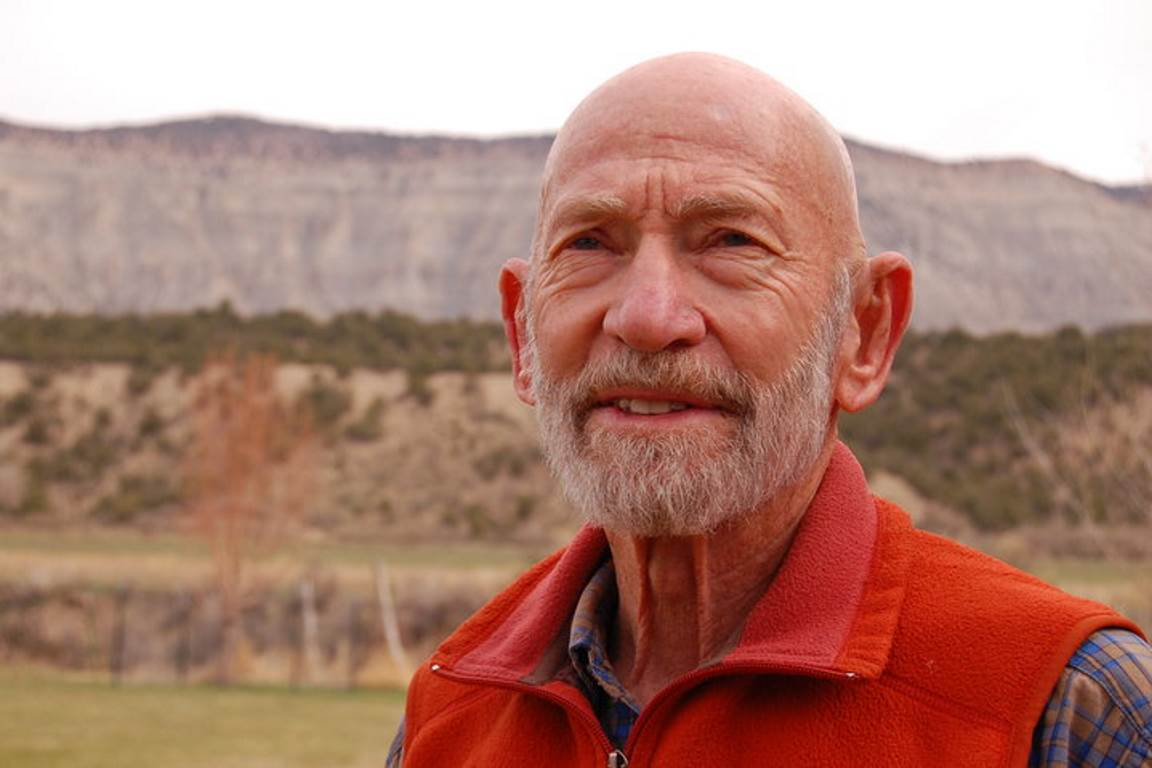
\includegraphics[keepaspectratio]{modulo1-resumo_files/mediabag/michael-soule2.jpg}}

}

\caption{\href{https://oeco.org.br/colunas/nerd-budista-pai-da-biologia-da-conservacao-a-vida-maravilhosa-de-michael-soule/}{Leia
o obituário de Michael Soulé escrito por Fernando Fernandes}}

\end{figure}%

Foi nesse contexto que Michael Soulé propôs, em 1985, a pergunta
fundadora do campo --- ``o que é biologia da conservação?'' ---
descrevendo-o como uma disciplina de crise, análoga à medicina de
emergência: obrigada a agir e a formular recomendações mesmo diante de
dados incompletos, o que gera uma tensão constitutiva entre rigor
científico e urgência prática. Essa proposta ganhou corpo institucional
rapidamente: a fundação da Society for Conservation Biology (SCB) em
1987, o lançamento do periódico \emph{Conservation Biology} em 1988 e a
subsequente proliferação de programas de pós-graduação dedicados ao tema
já no início dos anos 1990 consolidaram, em um intervalo notavelmente
curto, uma comunidade científica com identidade própria (Meine et al.,
2006).

Meine, Soulé e Noss (2006) descrevem essa consolidação como o surgimento
de uma disciplina ``orientada por missão'' (\emph{mission-driven}),
característica que a distingue de campos puramente descritivos: seu
critério de sucesso não é apenas a produção de conhecimento, mas sua
aplicação efetiva à proteção da diversidade biológica da Terra. Essa
orientação normativa --- a ciência a serviço de um objetivo de
conservação explícito --- é um traço definidor que atravessa toda a
história subsequente do campo, e que o aproxima de outras disciplinas
aplicadas, como a medicina ou a agronomia, nas quais o compromisso com
um resultado prático coexiste, nem sempre sem tensão, com os critérios
convencionais de objetividade científica.

\section{Raízes Filosóficas e a Ciência da Escassez e Abundância
(Terça-feira,
tarde)}\label{rauxedzes-filosuxf3ficas-e-a-ciuxeancia-da-escassez-e-abunduxe2ncia-teruxe7a-feira-tarde}

As raízes intelectuais da conservação são bem anteriores à sua
institucionalização científica. Tradições filosóficas ocidentais
convivem, desde o século XIX, em uma tensão nunca inteiramente resolvida
entre visões utilitaristas --- que tratam a natureza como um recurso a
ser gerido racionalmente --- e visões que lhe atribuem valor intrínseco,
independente de qualquer utilidade humana. Essa segunda corrente
encontra expressão emblemática na ``ética da terra'' proposta por
\href{https://pt.wikipedia.org/wiki/Aldo_Leopold}{Aldo Leopold} em
\emph{A Sand County Almanac} (1949), que defendia a ampliação da
comunidade moral para incluir solos, águas, plantas e animais, e nos
escritos de
\href{https://www.nytimes.com/2020/07/22/us/sierra-club-john-muir.html}{John
Muir}, um notótio racista e supremacista branco, cuja defesa de uma
natureza intocada, de valor estético e espiritual, se contrapunha à
visão conservacionista de uso racional de recursos defendida por
\href{https://pt.wikipedia.org/wiki/Gifford_Pinchot}{Gifford Pinchot}.

Essa disputa filosófica teve consequência institucional direta na
criação, em 1872, do Parque Nacional de Yellowstone --- o primeiro do
mundo --- que consolidou um modelo específico de área protegida: um
espaço \emph{supostamente desabitado}, preservado por seu valor estético
e recreativo \emph{para populações urbanas}. Esse modelo se espalharia
pelo mundo ao longo do século XX como padrão praticamente universal de
conservação, moldando não apenas a criação de parques nos Estados
Unidos, mas também a legislação ambiental de dezenas de outros países,
incluindo o Brasil.

É precisamente nesse ponto que a narrativa convencional da disciplina
exige uma qualificação importante, retomada com mais profundidade na
próxima seção: essas tradições filosóficas e os modelos institucionais
que delas derivaram muitas vezes expressam privilégios sociais
específicos (Dyke \& Lamb, 2020). A pergunta sobre quem definia o que
devia ser preservado --- e para quem --- carrega, desde a origem, uma
dimensão política que a narrativa estritamente biológica do campo tende
a deixar implícita.

\section{Uma genealogia também escrita a partir do Sul: Perspectivas
Latino-Americanas}\label{uma-genealogia-tambuxe9m-escrita-a-partir-do-sul-perspectivas-latino-americanas}

A narrativa até aqui apresentada --- de Soulé à fundação da SCB ---
descreve com precisão como a biologia da conservação se
institucionalizou nos Estados Unidos. Mas essa não é a única história
possível sobre a proteção da biodiversidade no mesmo período. Autores
latino-americanos, escrevendo majoritariamente em português e espanhol,
construíram paralelamente uma genealogia distinta, menos centrada na
consolidação disciplinar dentro da biologia e mais atenta aos conflitos
distributivos, às populações tradicionais e às disputas de poder
envolvidas na definição do que conta como ``natureza a ser protegida''.

O antropólogo brasileiro Antonio Carlos Diegues oferece a crítica mais
direta ao modelo institucional descrito na seção anterior. Em \emph{O
mito moderno da natureza intocada}, Diegues (2008) argumenta que a
concepção de áreas naturais protegidas como espaços desabitados e
intocados, herdada do modelo Yellowstone, constitui um mito de origem
especificamente europeia e norte-americana --- e que sua transposição
para países do que o autor chama do Sul Global produziu,
sistematicamente, a expulsão de populações tradicionais e indígenas de
seus territórios ancestrais, sem qualquer consideração pela história de
ocupação e manejo que essas populações mantinham com o ambiente. Para
Diegues, essa transposição ignora que a própria noção de ``natureza
selvagem'' (\emph{wilderness}) é uma construção cultural específica, e
não uma categoria universalmente válida --- argumento que dialoga
diretamente com o modelo de exclusão discutido na próxima sessão do
módulo, sobre a evolução do conceito humano-natureza.

Enquanto a narrativa estadunidense localiza a origem da disciplina em
uma resposta relativamente recente (anos 1970-80) à crise de
biodiversidade, o economista e sociólogo ambiental hispano-mexicano
Enrique Leff situa a ecologia política latino-americana como um campo
que já se articulava desde a década de 1970, não como uma importação do
ambientalismo do Norte, mas como resposta a conflitos socioambientais
próprios da região, gerados pela racionalidade do mercado e por
dinâmicas de exploração de recursos herdadas de processos coloniais e
pós-coloniais (2003). Leff argumenta que a ecologia política
latino-americana nasce de uma diferenciação epistemológica explícita
entre o ecologismo das sociedades já industrializadas --- que ele
descreve como um ``ecologismo pós-material'', voltado a preocupações
estéticas e de qualidade de vida --- e o que chama de ``ecologismo dos
pobres'', ancorado na sobrevivência material de populações que dependem
diretamente dos recursos ambientais em disputa.

Essa mesma distinção é desenvolvida com profundidade pelo economista
ecológico Joan Martínez-Alier, cuja obra é amplamente lida e debatida em
toda a América Latina. Em \emph{El ecologismo de los pobres},
Martínez-Alier (2004) documenta uma multiplicidade de conflitos
ecológicos distributivos ao redor do mundo --- muitos deles
latino-americanos --- nos quais populações marginalizadas mobilizam-se
em defesa de recursos ambientais dos quais depende sua própria
sobrevivência. O argumento central do autor inverte um pressuposto comum
na literatura ambientalista do Norte: o meio ambiente não é um luxo
pós-material que sociedades ricas podem se dar ao luxo de valorizar, mas
uma necessidade material imediata para os mais pobres. Essa formulação
oferece um contraponto direto à trajetória disciplinar descrita nas
seções anteriores, que emerge justamente de uma sociedade
industrializada e relativamente próspera.

Uma quarta contribuição, da antropóloga colombiana Astrid Ulloa,
adiciona uma camada crítica adicional a essa genealogia. Em \emph{La
construcción del nativo ecológico}, Ulloa (2004) analisa como o discurso
ambientalista internacional passou a construir povos indígenas como
guardiões ecológicos ``naturais'' de seus territórios --- uma identidade
que, segundo a autora, confere capital político e acesso a financiamento
internacional a esses povos, mas que simultaneamente corre o risco de
essencializar e imobilizar identidades indígenas em uma imagem estática,
ignorando suas próprias transformações internas, contradições e
diversidade de posições políticas. A crítica de Ulloa é útil
precisamente porque não endossa acriticamente a narrativa de
resistência: ela mostra que a aliança entre movimentos indígenas e
ambientalismo internacional é, ela mesma, um campo de disputa política,
não uma harmonia pré-existente.

Lidas em conjunto, essas quatro contribuições --- Diegues, Leff,
Martínez-Alier e Ulloa --- não substituem a narrativa institucional
apresentada nas seções anteriores; elas a colocam em perspectiva.
Enquanto a biologia da conservação, tal como narrada por Meine, Soulé e
Noss, nasce de uma comunidade científica relativamente homogênea,
concentrada em universidades e sociedades científicas do hemisfério
Norte, a ecologia política latino-americana nasce de conflitos
distributivos concretos, movimentos sociais e disputas territoriais, com
pouca ou nenhuma referência à sociedade acadêmica que fundou a SCB.
Essas duas genealogias coexistiram por décadas, praticamente sem diálogo
direto, e é apenas a partir dos anos 2000 que a disciplina científica
começaria a incorporar, de forma mais sistemática, as questões que a
ecologia política latino-americana já vinha discutindo desde os anos
1970 --- como veremos na próxima seção.

\section{A Evolução do Conceito Humano-Natureza (Quinta-feira,
manhã)}\label{a-evoluuxe7uxe3o-do-conceito-humano-natureza-quinta-feira-manhuxe3}

Um dos deslocamentos mais significativos na história da disciplina foi a
revisão do papel atribuído aos seres humanos nos sistemas que ela busca
proteger. Nas formulações iniciais, herdeiras diretas do modelo
Yellowstone discutido acima, humanos apareciam predominantemente como
agentes externos de perturbação --- fontes de ameaça a serem contidas ou
excluídas das áreas protegidas. Esse modelo de exclusão gerou, como já
indicado pela crítica de Diegues, deslocamentos concretos de populações
tradicionais em diversos países, incluindo o Brasil, sobretudo nas
décadas em que a maior parte das unidades de conservação restritivas do
país foi criada.

Com o tempo, essa compreensão ampliou-se para reconhecer humanos também
como beneficiários dos serviços ecossistêmicos e como participantes
ativos dentro dos próprios sistemas ecológicos, um deslocamento
conceitual associado à emergência de noções como Antropoceno e sistemas
socioecológicos acoplados (Teel et al., 2018). O próprio conceito de
Antropoceno, entretanto, permanece controverso: há debate tanto sobre
seu marco temporal de início --- a Revolução Industrial, a era atômica
ou os processos de colonização das Américas são candidatos concorrentes
--- quanto sobre sua utilidade analítica, já que ele pode obscurecer a
enorme desigualdade entre os grupos humanos responsáveis pelos impactos
ambientais globais e aqueles que mais sofrem suas consequências, um
ponto que aproxima diretamente essa discussão do ``ecologismo dos
pobres'' de Martínez-Alier.

Essa mudança não foi apenas semântica. Ela expressa o reconhecimento,
cada vez mais consensual dentro do campo, de que os problemas centrais
da conservação são inerentemente sociais, e que a disciplina, apesar de
suas raízes epistemológicas nas ciências naturais, precisava incorporar
as ciências sociais para cumprir sua própria missão (Teel et al., 2018).
Paralelamente, a disciplina passou a se afastar da lógica de proteger a
natureza \emph{das} pessoas para buscar formas de protegê-la \emph{para}
as pessoas --- um princípio que se tornaria central nos debates sobre
reservas extrativistas, desenvolvimento integrado e direitos de povos
indígenas, explorados no Módulo 5 (Dyke \& Lamb, 2020). Vale notar, no
entanto, que essa reformulação --- ``proteger para'' as pessoas ---
precisa ser lida à luz da advertência de Ulloa: o reconhecimento do
papel dos povos tradicionais na conservação não é isento de disputas
políticas sobre quem fala em nome de quem, e sobre os riscos de reduzir
identidades indígenas complexas a uma função ecológica instrumental.

\section{Da Biologia da Conservação à Ciência da Conservação
(Quinta-feira,
tarde)}\label{da-biologia-da-conservauxe7uxe3o-uxe0-ciuxeancia-da-conservauxe7uxe3o-quinta-feira-tarde}

Passadas mais de duas décadas da pergunta seminal de Michael Soulé,
Kareiva e Marvier (2012) revisitam a questão em um contexto global já
reconhecidamente dominado pela ação humana. Os autores propõem que o
campo se ampliou para uma ``ciência da conservação'' interdisciplinar,
que assume explicitamente o acoplamento entre sistemas sociais e
naturais como premissa metodológica, e não apenas como consideração
adicional.

Essa ciência da conservação ampliada passa a incorporar prioridades até
então marginais dentro da disciplina científica estadunidense: atuar
dentro de paisagens produtivas (e não apenas em áreas protegidas
isoladas), reconstruir apoio público ao redor de suas causas, dialogar
com o setor corporativo e dar atenção mais sistemática a direitos
humanos e equidade (Kareiva \& Marvier, 2012). É digno de nota que essas
mesmas prioridades --- equidade, atenção às populações que dependem
diretamente dos recursos, crítica à separação entre áreas protegidas e
paisagens habitadas --- já vinham sendo formuladas pela ecologia
política latino-americana desde pelo menos os anos 1980, décadas antes
de sua incorporação pela ciência da conservação de língua inglesa. Essa
defasagem cronológica não é um detalhe menor: ela sugere que a
``novidade'' da ciência da conservação, do ponto de vista estadunidense,
correspondia, do ponto de vista latino-americano, à redescoberta tardia
de questões que os movimentos sociais e a academia da região já
colocavam havia tempo.

A proposta de Kareiva e Marvier não é, contudo, consensual. Ela gerou um
debate ainda em curso entre uma corrente mais tradicional, que preserva
o foco na proteção de áreas e espécies por seu valor intrínseco, e a
chamada \emph{new conservation}, mais disposta a priorizar o bem-estar
humano como parte constitutiva da missão conservacionista --- debate que
ecoa, ainda que em termos distintos, a disputa entre Muir e Pinchot
apresentada anteriormente. O argumento central de Kareiva e Marvier ---
de que estratégias de conservação devem maximizar simultaneamente a
preservação da biodiversidade e o bem-estar humano --- antecipa
diretamente as tensões entre ecologia e justiça social que estruturam os
módulos finais da disciplina.

\section{Considerações Finais}\label{considerauxe7uxf5es-finais}

A trajetória reconstruída neste módulo mostra que a biologia da
conservação nunca foi um campo estático nem singular: de uma disciplina
de crise fundamentada quase exclusivamente em biologia básica, ela se
reconfigurou, em poucas décadas, em um empreendimento interdisciplinar
que assume a inseparabilidade entre sistemas humanos e naturais. Mas
essa trajetória, quando contada apenas a partir de sua
institucionalização estadunidense, permanece incompleta. A leitura
paralela de Diegues, Leff, Martínez-Alier e Ulloa revela uma segunda
genealogia --- latino-americana, articulada em português e espanhol,
nascida de conflitos distributivos concretos e da crítica ao modelo de
área protegida herdado de Yellowstone --- que antecipou, muitas vezes
por décadas, questões que a disciplina científica de língua inglesa
levaria até os anos 2010 para incorporar de forma sistemática.

Essa dupla genealogia é a chave de leitura para os módulos seguintes,
que aprofundarão, respectivamente, o desenvolvimento da disciplina no
Brasil --- onde essas duas tradições se encontram de forma
particularmente direta ---, a dimensão biológica da biodiversidade, a
interdisciplinaridade com as ciências humanas e a articulação da
conservação com a ecologia política.

\protect\phantomsection\label{refs}
\begin{CSLReferences}{1}{0}
\bibitem[\citeproctext]{ref-diegues2008}
Diegues, A. C. (2008). \emph{O mito moderno da natureza intocada} (6.ª
ed.). Hucitec/NUPAUB-USP.

\bibitem[\citeproctext]{ref-dyke2020}
Dyke, F., \& Lamb, R. (2020). \emph{The History and Distinctions of
Conservation Biology}. \url{https://doi.org/10.1007/978-3-030-39534-6_1}

\bibitem[\citeproctext]{ref-kareiva2012}
Kareiva, P., \& Marvier, M. (2012). What is Conservation Science?
\emph{BioScience}, \emph{62}(11), 962--969.
\url{https://doi.org/10.1525/bio.2012.62.11.5}

\bibitem[\citeproctext]{ref-leff2003}
Leff, E. (2003). \emph{Ecología Política: una perspectiva
latinoamericana}.
\url{https://www.redcolca.org/wp-content/uploads/Leff-Ecologia-Politica-Una-perspectiva-latinoamericana.pdf}

\bibitem[\citeproctext]{ref-martinezalier2004}
Martínez-Alier, J. (2004). \emph{El ecologismo de los pobres: conflictos
ambientales y lenguajes de valoración}. Icaria/FLACSO.

\bibitem[\citeproctext]{ref-meine2006}
Meine, C., Soulé, M., \& Noss, R. (2006). "A Mission-Driven Discipline":
the Growth of Conservation Biology. \emph{Conservation Biology},
\emph{20}. \url{https://doi.org/10.1111/j.1523-1739.2006.00449.x}

\bibitem[\citeproctext]{ref-teel2018}
Teel, T. L., Anderson, C. B., Burgman, M., Cinner, J., Clark, D.,
Estévez, R. A., Jones, J. P. G., McClanahan, T., Reed, M. S., Sandbrook,
C., \& St. John, F. (2018). Publishing social science research in
Conservation Biology to move beyond biology. \emph{Conservation
Biology}, \emph{32}. \url{https://doi.org/10.1111/cobi.13059}

\bibitem[\citeproctext]{ref-ulloa2004}
Ulloa, A. (2004). \emph{La construcción del nativo ecológico:
complejidades, paradojas y dilemas de la relación entre los movimientos
indígenas y el ambientalismo en Colombia}. ICANH/Colciencias.

\end{CSLReferences}




\end{document}
